\documentclass[a4paper]{article}
\usepackage{graphicx,tikz} 
\usepackage{multirow}
\usepackage{enumitem}
\usepackage{amssymb}
\usepackage{amsmath}
\usepackage{amsthm}
\usepackage{xcolor}
\usepackage{multicol}
\usepackage{multirow}
\usepackage{array}
\usepackage{animate}
\usepackage{amsthm}
\usepackage{caption}
\usepackage{minted}
\usepackage{fancyhdr}
\usepackage{geometry}
	\geometry{
		total = {160mm, 237mm},
		left = 30mm,
		right = 35mm,
		top = 35mm,
        bottom = 30mm,
        headheight=2cm
	}
\renewcommand{\headrulewidth}{0pt}

\graphicspath{{C:/Users/teoso/OneDrive/Documents/Tugas Kuliah/Template Math Depart/}}

\newcommand{\R}{\mathbb{R}}
\newcommand{\N}{\mathbb{N}}
\newcommand{\Z}{\mathbb{Z}}
\newcommand{\Q}{\mathbb{Q}}
\newcommand{\jawab}{\textbf{Solusi}:}

\title{Soal OSK Informatika}
\author{Permutasi dan Kombinasi}
\date{8 Maret 2025}

\begin{document}

\maketitle

\begin{enumerate}
  \item\textbf{(OSK 2022)} Tahun ini Pak Dengkleh ditunjuk menjadi ketua panitia Olimpiade Internasional Bebek (OIB). Untuk memberikan pengalaman kepada bebek-bebeknya, Pak Dengkleh berencana memilih 10 dari 15 bebek yang dimilikinya untuk menjadi peserta. Tentunya kita tahu bahwa di antara 15 bebek tersebut, ada empat bebek kesayangan Pak Dengkleh, yaitu Kwak, Kwik, Kwek, dan Kwok. Kwak dan Kwik harus dipilih untuk menjadi peserta lomba karena keduanya yang paling pintar. Sedangkan Kwek dan Kwok tidak bisa dipilih sebab saat ini sedang sakit. Ada berapa banyak cara memilih bebek-bebek sebagai peserta OIB?

  \begin{itemize}
      \item[A.] 303
      \item[B.] 286
      \item[C.] 196
      \item[D.] 165
      \item[E.] 120
  \end{itemize}

  \item\textbf{(OSK 2022)} Jika diberikan sembilan buah patok pada lahan Pak Dengklek sebagai berikut:

\begin{center}
    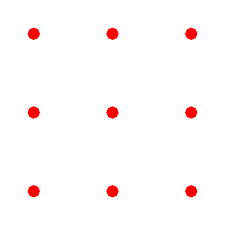
\begin{tikzpicture}
        \foreach \x in {0,1,2} {
            \foreach \y in {0,1,2} {
                \filldraw[red] (\x, \y) circle (2pt);
            }
        }
    \end{tikzpicture}
\end{center}

Pak Dengklek ingin membuat sebuah kandang yang berbentuk segitiga dimana setiap pojok sudut kandang harus merupakan patok-patok tersebut. Sisi kandang boleh melewati atau mengandung patok-patok lainnya. Ada berapa banyak kemungkinan kandang yang bisa dibangun oleh Pak Dengklek?\\
Jawaban: ............ \textit{(tuliskan jawaban dalam bentuk ANGKA saja)}

  \item\textbf{(OSK 2023)} Karena merasa bebeknya sudah terlalu banyak, Pak Dengkleh ingin mengurangi jumlah bebeknya dengan cara menjual semua bebek yang tidak ‘unggul’. Pak Dengkleh menyiapkan 10 soal dari nomor 1 sampai 10 untuk dikerjakan semua bebeknya (benar bernilai 1, salah bernilai 0). Bebek dikatakan `unggul' jika mendapat nilai paling sedikit 8. Kwak adalah bebek yang sangat cerdas dan telah mengetahui jawaban yang benar dalam menjawab soal apapun. Namun, Kwak tidak selalu ingin memberikan jawaban yang benar. Agar Kwak tidak dijual, berapa banyaknya cara Kwak memilih soal yang akan dijawab dengan benar jika Kwak menjawab soal nomor 1, 3, dan 5 dengan benar?

\begin{itemize}
    \item[A.] 29
    \item[B.] 21
    \item[C.] 8
    \item[D.] 3
    \item[E.] 1
\end{itemize}

    \item\textbf{(OSK 2024)} Perhatikan potongan kode program berikut.
    \begin{minted}[fontsize=\normalsize,frame=lines,framesep=2mm,linenos]{cpp}
bool cek(string S) {
    int n = S.length();
    for (int i = 0; i < n-1; i++) {
        if (S[i] > S[i+1]) return false;
    }
    return true;
}
    \end{minted}
    Jika \texttt{S} adalah sebuah string dengan panjang 3 dan hanya terdiri dari huruf kapital \texttt{`A'} hingga \texttt{`Z'}, maka berapa banyak kemungkinan \texttt{S} sedemikian sehingga pemanggilan \texttt{cek(S)} mengembalikan \textbf{\texttt{TRUE}}? \\
    Jawaban: ............ \textit{(tuliskan jawaban dalam bentuk ANGKA saja)}

\item\textbf{(OSK 2024)} Perhatikan potongan kode program berikut.
    \begin{minted}[fontsize=\normalsize,frame=lines,framesep=2mm,linenos]{cpp}
int panas(int X) {
     if (X == 0) return 0;
     else return (X % 10) + panas(X / 10);
}
int dingin(int X, int Y) {
     int air = 0;
     while (panas(air) != X) air = air + Y;
     return air; 
}
    \end{minted}
Berapa banyak pasang \texttt{<X,Y>} berbeda sehingga kembalian dari pemanggilan \texttt{dingin(X,Y)} adalah \texttt{77}?\\
Jawaban: ............ \textit{(tuliskan jawaban dalam bentuk ANGKA saja)}

\item\textbf{(OSK 2024)} Perhatikan potongan kode program berikut.

\begin{minted}[fontsize=\normalsize,frame=lines,framesep=2mm,linenos]{cpp}
bool dua_mata(vector<int> A, int kiri, int kanan) {
    if (kiri == kanan) {
        return (A[kiri] == 0);
    } else {
        int mid = (kiri + kanan) / 2;
        if (A[mid] < 0) {
            return dua_mata(A, kiri, mid-1);
        } else if (A[mid] > 0) {
            return dua_mata(A, mid+1, kanan);
        } else {
            return false;
        }
    }
}
\end{minted}

\noindent Dari 5 pilihan pemanggilan berikut, manakah yang hasil kembaliannya adalah \texttt{\textbf{TRUE}}?

\begin{enumerate}[label=\Alph*.]
    \item \texttt{dua\_mata(\{0,1,2,3,4,5,6\}, 0, 6)}
    \item \texttt{dua\_mata(\{-2,-1,0,1,2,3,4\}, 0, 6)}
    \item \texttt{dua\_mata(\{4,3,2,1,0,-1,-2\}, 0, 6)}
    \item \texttt{dua\_mata(\{6,-5,-4,-3,-2,-1,0\}, 0, 6)}
    \item \texttt{dua\_mata(\{-1,0,1,0,-1,0,1\}, 0, 6)}
\end{enumerate}

\noindent Jika \texttt{A} adalah sebuah vektor dengan panjang 7 dan hanya terdiri dari angka \texttt{-1}, \texttt{0}, atau \texttt{1}; maka berapa banyak vektor \texttt{A} berbeda sedemikian sehingga pemanggilan \texttt{\textbf{dua\_mata}(A,0,6)} mengembalikan \textbf{\texttt{TRUE}}?\\
Jawaban: ............ \textit{(tuliskan jawaban dalam bentuk ANGKA saja)}

\end{enumerate}


\end{document}
